\mbox{}


\chapter{Entrenamiento del modelo mediante Google Colab}
\label{ch:chapter2}
Dentro del entrenamiento de modelos Deep Learning, la velocidad es uno de los parámetros fundamentales.
Los modelos pueden requerir entradas de tamaño masivo en las que la capacidad de cómputo se torne clave para acelerar el proceso;
esto permite enfocarse plenamente en la mejora de rendimiento del modelo planteado.
El objetivo es evitar la posible espera que pueda producir volver a entrenar el mismo con distintos parámetros.
Con ello, se puede reajustar constantemente el modelo para encontrar el punto óptimo de manera ágil.
En este trabajo se va a entrenar un modelo de deep learning haciendo uso del framework de código abierto de TensorFlow\footnote{https://www.tensorflow.org/}, que está programada en el lenguaje de programación Python.
Éste incluye una API de Deep Learning llamada Keras, que será la que utilicemos.
El tipo de operaciones que requiere nuestra aplicación en la parte del tratamiento de imágenes, así como los procedimientos que realizan las redes neuronales para hacer sus cálculos son, en muchas ocasiones,
operaciones matriciales.
Nuestro objetivo será aprovechar al máximo el rendimiento que una GPU puede aportar en este tipo de operaciones, principalmente por su arquitectura de paralelización, idónea para este tipo de trabajo.
La ventaja que aporta frente a la CPU es la capacidad de cómputo con un mayor número de núcleos o cores (ver Figura\ref{fig:Arquitectura de paralelización de una GPU}), gracias a su conectividad por PCI express y el ancho de banda que esta proporciona.

\begin{figure}
    \centering
    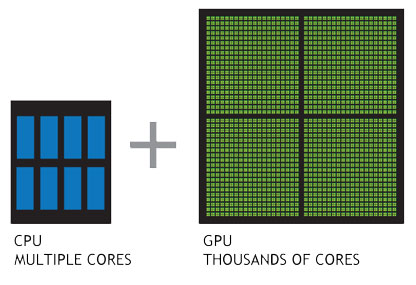
\includegraphics[width=0.5\textwidth]{images/chapter2/cpu-and-gpu.jpg}
    \caption{Arquitectura de paralelización de una GPU.}
    \label{fig:Arquitectura de paralelización de una GPU}
\end{figure}


\section{Modelo propuesto}\label{sec:modelo-propuesto}
En esta parte del trabajo se pretende conseguir la máxima velocidad de entrenamiento posible manteniendo unos niveles de precisión elevados en la predicción.
Nuestro modelo tiene como cometido primordial poder clasificar distintas imágenes según el estado del terreno que aparece en la fotografía, siendo las opciones: terreno dañado y terreno en buenas condiciones.
Para ello, disponemos de un dataset de 268 imágenes multiespectrales (describir dataset, procedencia).
Una imagen multiespectral es la que captura datos de imágenes dentro de rangos de longitud de onda específicos a través del espectro electromagnético.
Como framework principal para realizar el entrenamiento nos ayudaremos de TensorFlow, que incluye la librería de deep learning Keras,
la cual simplifica mucho la implementación de este tipo de algoritmos de aprendizaje automático, debido a que sus objetos y funciones están programados de una manera intuitiva.
La distribución a efectuar sobre el conjunto de datos en entrenamiento y test es del 70\% y 30\% respectivamente.
Para la construcción de este algoritmo haremos uso de las siguientes capas, sobre las que TensorFlow nos da una API para tener control total sobre su configuración.
\begin{itemize}
    \item \textbf{Conv2D}: Capa convolucional cuyo principal objetivo es extraer características de la imagen de entrada o partes de la misma.
    El térmido 2D se refiere al movimiento del filtro, el cuál es un parámetro de entrada de este tipo de capas.
    El filtro atraviesa la imagen en dos dimensiones.
    Tiene como parámetros de entrada una imagen en tres dimensiones y el número de filtros que vamos a aplicar sobre la imagen.
    Aplicaremos sobre esta capa una configuración de 64 filtros y un tamaño de kernel de 3x3 ya que nuestras imágenes son de 128x128 píxeles.Los filtros de mayor tamaño ayudarán al modelo a mejorar su aprendizaje.
    \item \textbf{Activación Relu (Recitified Linear Unit)}: En redes neuronales, una función de activación es la responsable de transformar la entrada.
    Sus principales funciones son detectar posibles correlaciones entre dos variables distintas dependiendo de sus valores y ayudar al modelo a tener en cuenta funciones no lineales, lo que significa, que la red neuronal es capaz de realizar microajustes para capturar relaciones entre entradas y salidas que no sigan una línea recta en el plano cartesiano.
    Como podemos observar en la figura~\ref{fig:Función de activación Relu} la función de activación Relu se comporta devolviendo un 0 para valores de entrada negativos y en caso contrario devolviendo el propio valor de entrada.
    Esta función de activación conserva los valores que contienen algún patrón en la imagen y los transfiere a la siguiente capa, mientras que los pesos negativos no son importantes y son establecidos con el valor 0.
    Otras funciones de activación como la función Sigmoide o Tanh modifican todos los valores de entrada, la función Relu mantendrá los valores de peso positivo para las capas posteriores.
    \item \textbf{MaxPooling2D}: Es una capa que sigue un proceso de discretización basado en muestras, su objetivo es reducir la muestra de una representación de entrada mediante el acortamiento de sus dimensiones.
    En nuestro modelo aplicaremos una reducción a matrices de 2x2.
    \item \textbf{Dropout}: Es una capa cuyo cometido es ignorar ciertas neuronas de forma aleatoria para no incluirlas en el entrenamiento, por lo que las neuronas restantes serán las encargadas de representar las predicciones de la red.
    De esta manera también reducimos la complejidad de nuestra red y la posibilidad de sobreentrenamiento.
    \item \textbf{Flatten}: Capa de aplanamiento usada para reducir a uno el número de dimensiones de nuestra matriz de entrada.
    \item \textbf{Dense}: Una de las capas más utilizadas en la API de Keras, es la manera de efectuar multiplicaciones matriciales.
    \item \textbf{Optimizador Adam}: Es un algoritmo de optimización diseñado especialmente para redes neuronales, este aprovecha el poder de los métodos de tasas de aprendizaje adaptativo para encontrar nivel de aprendizaje individuales para cada parámetro.
\end{itemize}

En la Figura~\ref{fig:Topología de la red del modelo de redes neuronales.} podemos observar el conjunto de capas utilizado para crear la topología de la red de nuestro modelo.
\begin{figure}
    \centering
    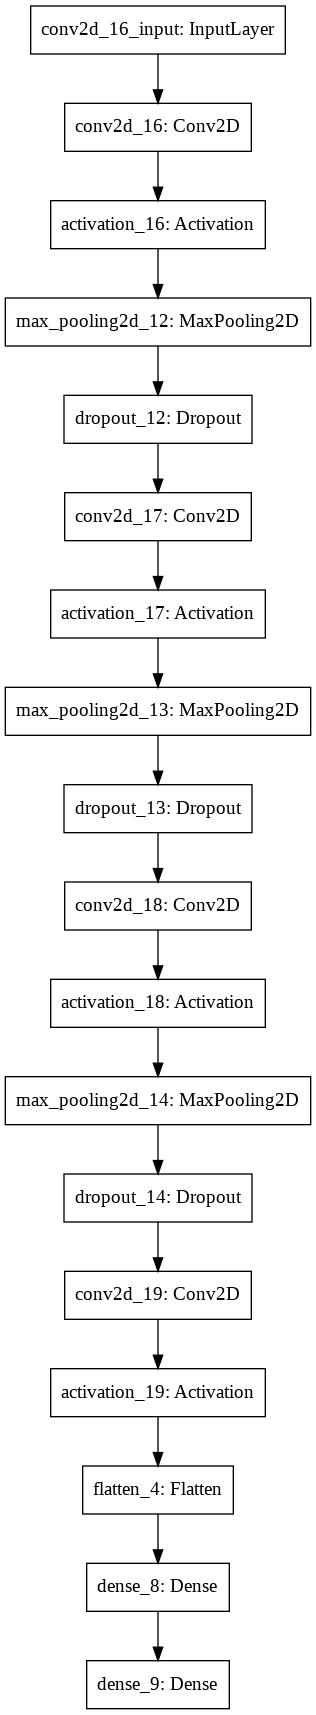
\includegraphics[width=0.2\textwidth]{images/chapter2/model.png}
    \caption{Topología de la red del modelo de redes neuronales.}
    \label{fig:Topología de la red del modelo de redes neuronales.}
\end{figure}

\begin{figure}
    \centering
    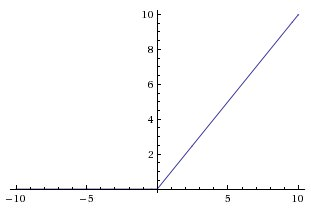
\includegraphics[width=0.5\textwidth]{images/chapter2/relu.jpg}
    \caption{Función de activación Relu.}
    \label{fig:Función de activación Relu}
\end{figure}
Además, realizaremos algunas optimizaciones a nivel de hardware para acelerar el proceso de forma general.

\begin{itemize}
    \item \textbf{Uso de variables de 16 bits en vez de 32 bits}: Una de las posibilidades que nos brinda el uso de una GPU es reducir a la mitad el uso en memoria de las variables del proceso.
    Usaremos esto siempre y cuando no afecte a la calidad de la predicción.
    \item \textbf{Uso del compilador XLA}: El compilador XLA (Accelerated Linear Algebra) optimiza el grafo de nuestro modelo de manera específica haciendo uso de la GPU.
    \item \textbf{Valores altos del parámetro de entrenamiento BatchSize}: Gracias a la capacidad de cómputo de nuestra tarjeta gráfica podemos permitirnos el uso de valores altos en este parámetro de entrenamiento.
\end{itemize}


\section{Entorno Google Colab}\label{sec:entorno-google-colab}
La plataforma de Google Colab\footnote{https://colab.research.google.com/notebooks/intro.ipynb} es un servicio gratuito de Google, mediante el cual podemos ejecutar e instalar librerías del lenguaje de programación Python.
Una de las grandes ventajas de trabajar con este entorno es que no necesitamos configuración ninguna, se ejecuta de forma íntegra en el navegador sin necesidad de instalar nada previamente y podemos compartir
nuestro trabajo con otras personas.
Estas características permiten a Google Colab convertirse en un entorno muy válido para personas que están dando sus primeros pasos en este área de la inteligencia artificial, pero haciendo uso
de unas herramientas profesionales.
En este trabajo haremos uso de la tarjeta gráfica Tesla K80.
Las características primarias de nuestra principal unidad de cómputo son las siguientes :
\begin{itemize}
    \item 4992 núcleos de NVIDIA CUDA con diseño de dos GPU\@.
    \item Hasta 2,91 teraflops de rendimiento en operaciones de precisión doble con NVIDIA GPU Boost.
    \item 24 GB de memoria GDDR5.
    \item 480 GB/s de ancho de banda de memoria agregado.
    \item Hasta 8,73 teraflops de rendimiento en operaciones de precisión simple con NVIDIA GPU Boost.
\end{itemize}
El uso de este tipo de herramientas en esta plataforma es extrapolable a otras nubes sin las restricciones en cuanto al número de unidades de procesamiento que necesitamos, la interoperabilidad de sus elementos con otros componentes externos, tales como servidores o respositorios de código, así como la configuración explícita de cada uno de los entornos de ejecución.
Una de las principales ventajas que tiene poder usar un entorno como Google Colab es que el servicio se ejecuta de manera íntegra online, de modo que toda la carga computacional reside en la herramienta de Google y no en nuestro computador.
Esto permite trabajar de manera fluida realizando otro tipo de cometidos en nuestra máquina, o simplemente ejecutar un proceso para el que no tenemos suficiente potencia disponible.
